\documentclass[12pt]{exam}		%Doc : https://mirrors.ircam.fr/pub/CTAN/macros/latex/contrib/exam/examdoc.pdf
\printanswers					%Comment this line to hide the answers 
\usepackage[utf8]{inputenc}
\usepackage[T1]{fontenc}
\usepackage[french]{babel}      %Originally for french document, change to english or relevant language

\usepackage{amsmath,amssymb}
\usepackage{multicol}
\usepackage[dvipsnames]{xcolor}
\usepackage[shortlabels]{enumitem}
\usepackage{tikz}
	\usetikzlibrary{fadings}
	\usetikzlibrary{calc}
	
\usepackage{tkz-tab}
\usepackage{pgfplots}

%Format Header and footer
\pagestyle{headandfoot}
\header{\footnotesize Class\\Id number}{\Large\textbf{Name}}
\headrule
\footrule
\setlength{\columnsep}{0.25cm}
%\setlength{\columnseprule}{1pt}
\footer{}{Page \thepage}{}
%\extrafootheight{-2cm}

% Change section command behaviour
\usepackage{titlesec}
\titleformat{\section}[frame]{\Huge\bfseries\filright}{}{2mm}{\centering Chemistry 107 :\ }

% Add a watermark if answers are shown
%\ifprintanswers
%\usepackage{draftwatermark}
%\SetWatermarkColor{red!30}
%\SetWatermarkScale{5}
%\SetWatermarkText{Solution}     %Watermark text
%\fi

%Format the name of each exercise
\qformat{\textbf{Exercice \thequestion~:}\hfill}
\extrawidth{1.5cm}

\begin{document}
\section{Exam 3A}

\noindent The 100 pts exam consists of 9 questions and students have 2 hours to complete the exam.
Answers must be written in the box provided or else no credit is provided. Use the empty
space provided to do your work. A periodic table and formulas are provided at the end. Additional
scratch paper will be provided. Fill in your name along with your student ID number.
\\

\noindent\textbf{Problem 1: True/False } Determine whether the statement is true or false. (10 pts)
\\
\begin{enumerate}[(a)]
\item For an ideal gas, increasing the pressure decreases the volume. %True
\item[]\tikz[baseline=1ex]\draw (0,0) rectangle (17cm,5ex);
\item The second ionization energy of alkaline earth metals is higher than the
  second ionization energy of alkali metals. %False
\item[]\tikz[baseline=1ex]\draw (0,0) rectangle (17cm,5ex);
\item In a compound with resonance structures, the actual structure of the molecule is
  the average of all resonance structures. %True
\item[]\tikz[baseline=1ex]\draw (0,0) rectangle (17cm,5ex);
\item Lewis structures can predict the geometric shape of compounds. %False
\item[]\tikz[baseline=1ex]\draw (0,0) rectangle (17cm,5ex);
\item The atomic radius increases moving from the left to right on the
  periodic table. %False
\item[]\tikz[baseline=1ex]\draw (0,0) rectangle (17cm,5ex);
\item The electron configuration of molybdenum (Mo) is [Kr]5s$^2$4d$^4$. %False
\item[]\tikz[baseline=1ex]\draw (0,0) rectangle (17cm,5ex);
\item At each energy level, the multielectron orbital diagram shows
  that the atomic orbitals are nondegenerate. %True
\item[]\tikz[baseline=1ex]\draw (0,0) rectangle (17cm,5ex);
\item Chemical bonds are made of atomic orbitals. %True
\item[]\tikz[baseline=1ex]\draw (0,0) rectangle (17cm,5ex);
\item UV lights have lower energy than infrared. %False
\item[]\tikz[baseline=1ex]\draw (0,0) rectangle (17cm,5ex);
\item As the frequency of light increases, the photon energy increases
  as well %True
\item[]\tikz[baseline=1ex]\draw (0,0) rectangle (17cm,5ex);
\end{enumerate}

\newpage

\noindent\textbf{Problem 2: Boyle's Law} Given fixed amount of gas at constant
temperature. Answer the following questions and report to 3 significant figures.
(16 pts)

\begin{enumerate}[(a)]
\item A balloon contains 500.mL of helium when filled at 1.00atm. What would be
  the volume of the balloon if it were subjected to 5.50atm of pressure?
  \vspace{1in}
\item[]\tikz[baseline=1ex]\draw (0,0) rectangle (17cm,5ex);
\item What pressure is needed to compress 350mL of oxygen gas at 2.50atm to a volume
  of 75mL?
  \vspace{1in}
\item[]\tikz[baseline=1ex]\draw (0,0) rectangle (17cm,5ex);
\item A particular balloon is designed by its manufacturer to be inflated to a volume
  of no more than 2.5 liters. If the balloon is filled with 2.0 liters of helium at sea
  level (101.325 kPa), and rises to an altitude where the pressure is 89.1kPa, will the
  balloon burst?
  \vspace{1.4in}
\item[]\tikz[baseline=1ex]\draw (0,0) rectangle (17cm,5ex);
\item Draw the graph of the relationship between pressure (P) and volume (V).
  Describe the relationship.
\item[]\tikz[baseline=1ex]\draw (0,0) rectangle (17cm,30ex);
\end{enumerate}

\newpage

\noindent\textbf{Problem 3: Charles' Law} Given a fixed amount of gas at constant
pressure. Answer the following questions and report to 3 significant figures. (12 pts)

\begin{enumerate}[(a)]
\item If a sample of chlorine gas occupies 50.0mL at 100.$^\circ$C, what is its
  volume at 25.0$^\circ$C?
  \vspace{1.5in}
\item[]\tikz[baseline=1ex]\draw (0,0) rectangle (17cm,5ex);
\item Calculate the temperature (in Celsius) when 2.00L at 21.0$^\circ$C is
  compressed to 1.00L.
  \vspace{1.5in}
\item[]\tikz[baseline=1ex]\draw (0,0) rectangle (17cm,5ex);
\item Draw the graph of the relationship between volume (V) and temperature (T)
  for an ideal gas. Describe the relationship.
\item[]\tikz[baseline=1ex]\draw (0,0) rectangle (17cm,30ex);
\end{enumerate}

\newpage

\noindent\textbf{Problem 4: Avogadro's Hypothesis} At constant pressure and
temperature, answer the following questions and report to 3 significant figures.
(12 pts)

\begin{enumerate}[(a)]
\item If a 10.0L balloon contains 1.00mol of gas, what will be the volume of a balloon
  that contains 0.20mol of gas?
  \vspace{1.5in}
\item[]\tikz[baseline=1ex]\draw (0,0) rectangle (17cm,5ex);
\item A flexible container at an initial volume of 5.120L contains 8.500mol of gas.
  More gas is then added to the container until it reaches a final volume of 18.1L.
  Determine the total number of moles at 18.1L.
  \vspace{1.5in}
\item[]\tikz[baseline=1ex]\draw (0,0) rectangle (17cm,5ex);
\item Draw the graph of the relationship between volume (V) and mole of gas (n)
  for an ideal gas. Describe the relationship.
\item[]\tikz[baseline=1ex]\draw (0,0) rectangle (17cm,30ex);
\end{enumerate}

\newpage

\noindent\textbf{Problem 5: Photosynthesis - the Chloroplast} Photosynthesis
is a vital process providing organisms oxygen and food. Plants performs this vital
process using a protein called chlorophyll a. The protein absorbs mainly light at
430nm (violet) and and 662nm (red). Answer the following questions and report to
3 significant figures. (10 pts)

\begin{enumerate}[(a)]
\item Determine the energy in J of the violet (430nm) and red light (662nm) that
  chlorophyll a absorbs.
  \vspace{2.5in}
\item[]\tikz[baseline=1ex]\draw (0,0) rectangle (17cm,5ex);
\item How much energy is contained in one mole of photons for violet and red lights?
  \vspace{2.5in}
\item[]\tikz[baseline=1ex]\draw (0,0) rectangle (17cm,5ex);
\end{enumerate}

\newpage

\noindent\textbf{Problem 6: Energy from a Laser} In 2021, HiLASE Center broke the world
record developing the strongest high-energy laser that emits a wavelength of 1030nm.
Answer the following questions and report to 3 significant figures. (12 pts)

\begin{enumerate}[(a)]
\item Determine the energy of a single photon from 1030nm.
  \vspace{1.75in}
\item[]\tikz[baseline=1ex]\draw (0,0) rectangle (17cm,5ex);
\item A single laser pulse emits 145 Joules of energy. Determine how many
  photons that is.
  \vspace{1.75in}
\item[]\tikz[baseline=1ex]\draw (0,0) rectangle (17cm,5ex);
\item Compute the energy in J/mol of a mole of photon at 1030nm. Compare this energy
  to part b).
  \vspace{1.75in}
\item[]\tikz[baseline=1ex]\draw (0,0) rectangle (17cm,5ex);
\end{enumerate}

\newpage

\noindent\textbf{Problem 7: Drawing Lewis Structures}
Draw the Lewis structures for the following compounds, identify the
geometric shape, and whether the compound is polar or nonpolar. If there
are resonance structures, then include them in your answer.(12 pts)

\begin{enumerate}[(a)]
\item CO$_2$
\item[]\tikz[baseline=1ex]\draw (0,0) rectangle (17.5cm,34ex);
\item SCN$^-$ 
\item[]\tikz[baseline=1ex]\draw (0,0) rectangle (17.5cm,34ex);
\item BF$_3$
\item[]\tikz[baseline=1ex]\draw (0,0) rectangle (17.5cm,34ex);
\item NH$_3$
\item[]\tikz[baseline=1ex]\draw (0,0) rectangle (17.5cm,35ex);
\item PO$_4^{3-}$
\item[]\tikz[baseline=1ex]\draw (0,0) rectangle (17.5cm,35ex);
\item SO$_4^{2-}$
\item[]\tikz[baseline=1ex]\draw (0,0) rectangle (17.5cm,35ex);
\end{enumerate}

\newpage

\noindent\textbf{Problem 8: Periodic Properties} Rank the following
periodic properties. (8 pts)

\begin{enumerate}[(a)]
\item Rank elements from highest to lowest first ionization energy:
  F, Li, He, Mg, I %He, F, I, Li, Mg
\item[]\tikz[baseline=1ex]\draw (0,0) rectangle (17cm,5ex);
\item Rank elements from highest to lowest electronegativity:
  Li, Be, Se, O, F %F, O, Se, Be, Li
\item[]\tikz[baseline=1ex]\draw (0,0) rectangle (17cm,5ex);
\item Rank elements from largest to smallest atomic radius:
  He, H, K, F, I %K, I, F, H, He
\item[]\tikz[baseline=1ex]\draw (0,0) rectangle (17cm,5ex);
\item Ranking ions from largest to smeallest atomic radius:
  N$^{3-}$, I$^-$, Li$^+$, F$^-$, O$^{2-}$ % I-, N3-, O2-, F-, Li+
\item[]\tikz[baseline=1ex]\draw (0,0) rectangle (17cm,5ex);
\end{enumerate}

\noindent\textbf{Problem 9: Electron Configuration} Determine the electron
configurations for the following. (8 pts)

\begin{enumerate}[(a)]
\item Mg % [Ne]2s2
\item[]\tikz[baseline=1ex]\draw (0,0) rectangle (17cm,5ex);
\item S % [Ne]3s2 3p4
\item[]\tikz[baseline=1ex]\draw (0,0) rectangle (17cm,5ex);
\item Al$^{3+}$ %[Ne]
\item[]\tikz[baseline=1ex]\draw (0,0) rectangle (17cm,5ex);
\item Cr % [Ar]4s1 3d5
\item[]\tikz[baseline=1ex]\draw (0,0) rectangle (17cm,5ex);
\item Zn$^{2+}$ % [Ar]3d10
\item[]\tikz[baseline=1ex]\draw (0,0) rectangle (17cm,5ex);
\item Fe$^{2+}$ % [Ar]3d10
\item[]\tikz[baseline=1ex]\draw (0,0) rectangle (17cm,5ex);
\item Ag$^+$ % [Ar]3d10
\item[]\tikz[baseline=1ex]\draw (0,0) rectangle (17cm,5ex);
\item Gd % [Ar]3d10
\item[]\tikz[baseline=1ex]\draw (0,0) rectangle (17cm,5ex);
%\item Au % [Ar]3d10
%\item[]\tikz[baseline=1ex]\draw (0,0) rectangle (17cm,5ex);
%\item Pb$^{2+}$ % [Ar]3d10
%\item[]\tikz[baseline=1ex]\draw (0,0) rectangle (17cm,5ex);
\end{enumerate}

\newpage

\appendix

\section{Appendix 1 - Periodic Table}

\begin{center}
  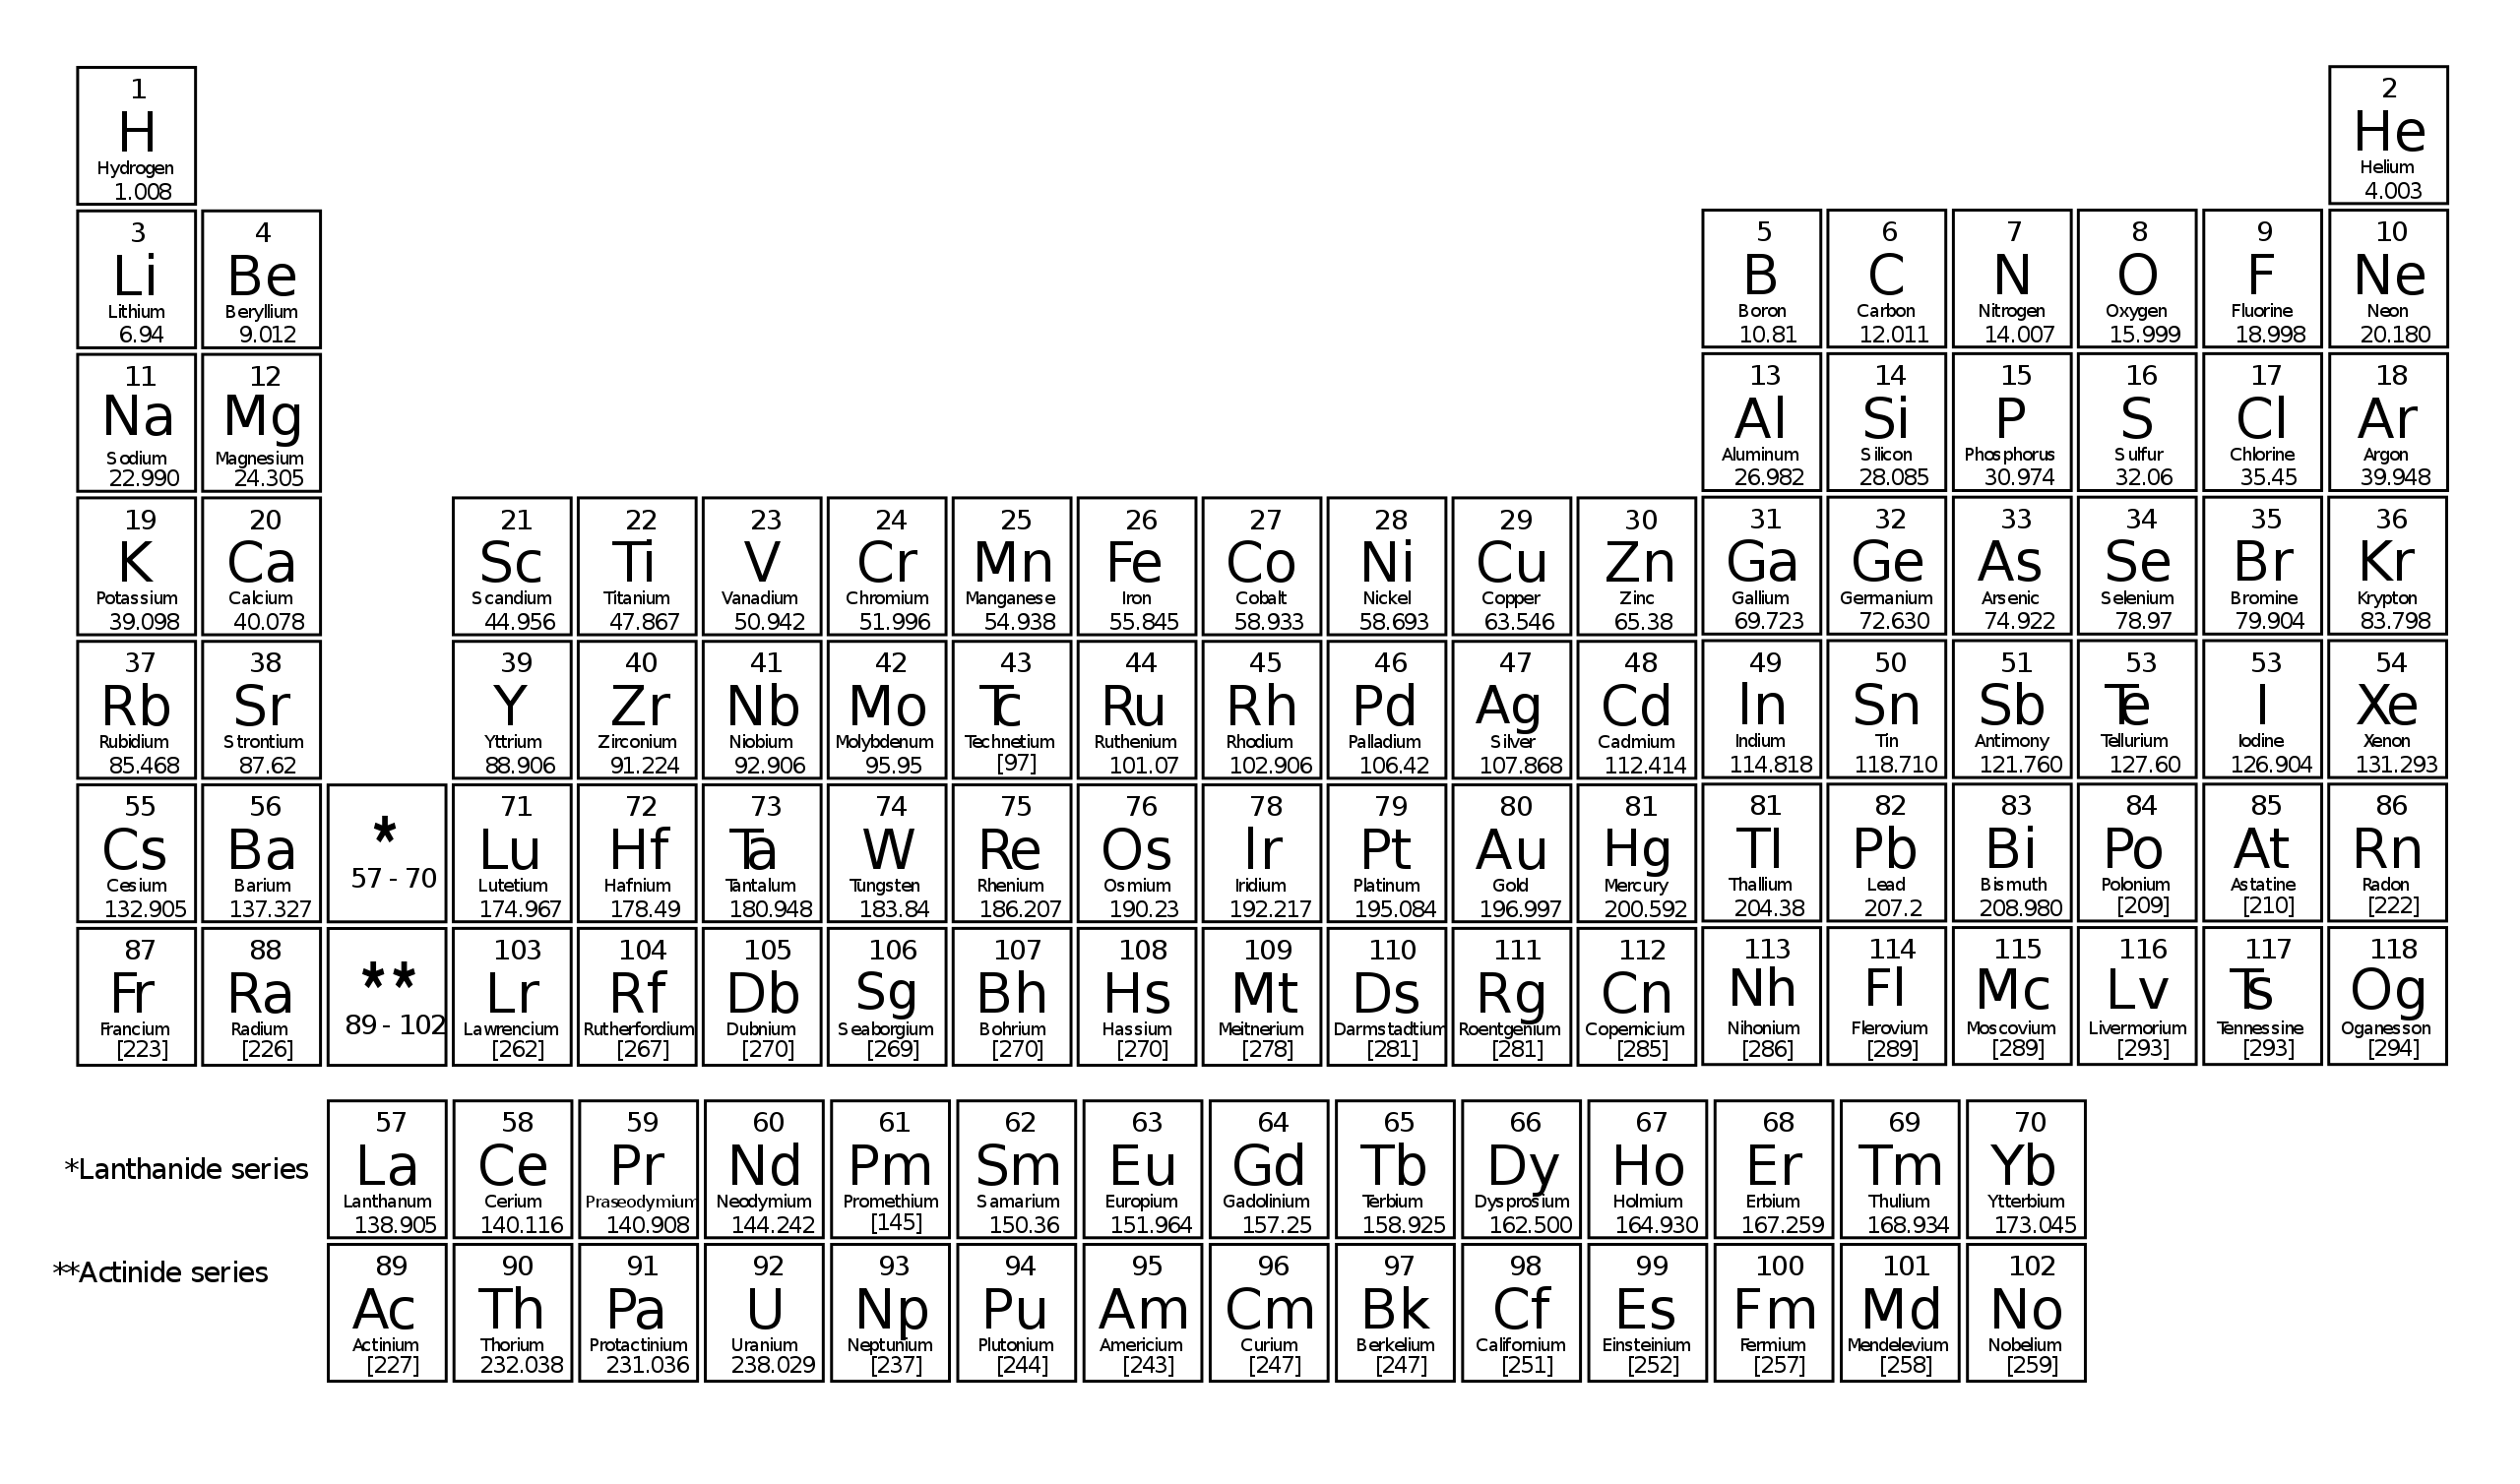
\includegraphics[scale=0.24,angle=90]{periodic_table}
\end{center}

\section{Apppendix 2 - Formulas and Constants}

\begin{align*}
  q = & mC\Delta T \\
  E = & \frac{hc}{\lambda} = h\nu \\
  h = & 6.626 \times 10^{-34} \text{J s} \\
  c = & \lambda \nu \\
  c = & 3.00 \times 10^8 \text{m/s} \\
  N_A = & 6.022\times 10^{23} \\
  P_1V_1 = & P_2V_2 \\
  \frac{V_1}{T_1} = & \frac{V_2}{T_2} \\
  \frac{P_1}{n_1} = & \frac{P_2}{n_2}
\end{align*}
\end{document}
